%%%%%%%%%%%%%%%%%%%%%%%%%%%%%%%%%%%%%%%%%
% Awesome Resume/CV
% XeLaTeX Template
% Version 1.3 (30/3/2020)
%
% This template has been downloaded from:
% http://www.LaTeXTemplates.com
%
% Original author:
% Claud D. Park (posquit0.bj@gmail.com) with modifications by 
% Vel (vel@latextemplates.com)
%
% License:
% CC BY-NC-SA 3.0 (http://creativecommons.org/licenses/by-nc-sa/3.0/)
%
% Important note:
% This template must be compiled with XeLaTeX, the below lines will ensure this
%!TEX TS-program = xelatex
%!TEX encoding = UTF-8 Unicode
%
%%%%%%%%%%%%%%%%%%%%%%%%%%%%%%%%%%%%%%%%%

%----------------------------------------------------------------------------------------
%	PACKAGES AND OTHER DOCUMENT CONFIGURATIONS
%----------------------------------------------------------------------------------------

\documentclass[11pt, a4paper]{awesome-cv} % A4 paper size by default, use 'letterpaper' for US letter
\usepackage{pdfpages}

\geometry{left=2cm, top=1.5cm, right=2cm, bottom=2cm, footskip=.5cm} % Configure page margins with geometry

\fontdir[fonts/] % Specify the location of the included fonts

% Color for highlights
\colorlet{awesome}{awesome-skyblue} % Default colors include: awesome-emerald, awesome-skyblue, awesome-red, awesome-pink, awesome-orange, awesome-nephritis, awesome-concrete, awesome-darknight
%\definecolor{awesome}{HTML}{CA63A8} % Uncomment if you would like to specify your own color

% Colors for text - uncomment and modify
%\definecolor{darktext}{HTML}{414141}
%\definecolor{text}{HTML}{414141}
%\definecolor{graytext}{HTML}{414141}
%\definecolor{lighttext}{HTML}{414141}

\renewcommand{\acvHeaderSocialSep}{\quad\textbar\quad} % If you would like to change the social information separator from a pipe (|) to something else

%----------------------------------------------------------------------------------------
%	PERSONAL INFORMATION
%	Comment any of the lines below if they are not required
%----------------------------------------------------------------------------------------

\name{}{Alireza Zakeri}
\address{Antwerpen, Belgium}
\mobile{+32472897157}

\email{Alireza\_zak@yahoo.com}
%\homepage{www.posquit0.com}
%\github{Alirezazak}
\linkedin{Alireza-Zakeri-a5b40587}{Alireza Zakeri}
%\stackoverflow{SOid}{SOname}
%\twitter{@twit}
%\reddit{reddit account}
%\xing{xing name}
%\extrainfo{test} % Other text you want to include on this line

\position{Embedded System Developer Engineer{\enskip\cdotp\enskip}Hardware Designer on FPGAs} % Your expertise/fields
%\quote{``Make the change that you want to see in the world."} % A quote or statement

\makecvfooter{\today}{Alireza Zakeri~~~·~~~Résumé}{\thepage} % Specify the letter footer with 3 arguments: (<left>, <center>, <right>), leave any of these blank if they are not needed

%----------------------------------------------------------------------------------------

\begin{document}

\makecvheader[R] % Print the header

%----------------------------------------------------------------------------------------
%	CV/RESUME CONTENT
%	Each section is imported separately, open each file in turn to modify content
%----------------------------------------------------------------------------------------

%-------------------------------------------------------------------------------
%	SECTION TITLE
%-------------------------------------------------------------------------------
\cvsection{Summary}


%-------------------------------------------------------------------------------
%	CONTENT
%-------------------------------------------------------------------------------
\begin{cvparagraph}

Qualified embedded system developer engineer with 4+ years experience specializing in HDL circuit design and real-time processor-based systems development. Familiar with customization of some OS types and hands-on many low-rate and high-rate protocols, processors, and microcontrollers programming. Eager to collaborate and work in a team, interested in devising a better problem-solving method for challenging tasks, and learning new technologies and tools if the need arises.
\end{cvparagraph}

%----------------------------------------------------------------------------------------
%	SECTION TITLE
%----------------------------------------------------------------------------------------

\cvsection{Skills}

%----------------------------------------------------------------------------------------
%	SECTION CONTENT
%----------------------------------------------------------------------------------------

\begin{cvskills}

%------------------------------------------------

\cvskill
{Hardware Development} % Category
{
\item Expert on hardware development by VHDL on Xilinx FPGAs (7 series and Ultra Scale).
\item Familiar with HDL design challenges such as timing faults and resolve..
\item Had experiences in debugging and test challenges in HDL designs.
\item Familiar with Analog Devices ADCs, STM32, and Atmel microcontrollers and their peripherals configuration (UART, I2C, SPI, and etc).
}

%------------------------------------------------

\cvskill
{System Development} % Category
{
\item Development and customization of Linux kernel, U-Boot, RTOS and firmware on Xilinx and TI SoCs (Zynq, ZynqMP, Keystone I\&II and Sitara).
\item Familiar with Linux devicetree structure and development driver in kernel.
\item Familiar with Yocto Project build system, rootfs customization and Jenkins pipeline.
\item Had a study on network concepts and protocols such as TCP/IP.
}

%------------------------------------------------

\cvskill
{Softwares} % Category
{C, Git, MATLAB, OpenCl}

%------------------------------------------------

\cvskill
{Personal Skills} % Category
{Punctuality, Teamwork, Flexibility and Adaptability} % Skills

%------------------------------------------------

\cvskill
{Languages} % Category
{Persian (native), English (fluent)} % Skills

%------------------------------------------------

\end{cvskills}

%----------------------------------------------------------------------------------------
%	SECTION TITLE
%----------------------------------------------------------------------------------------

\cvsection{Experience}

%----------------------------------------------------------------------------------------
%	SECTION CONTENT
%----------------------------------------------------------------------------------------

\begin{cventries}

%---------------------------------------------------------
  \cventry
  {Consultant (full-time)} % Job title
  {Dekimo Experts Gent} % Organization
  {Gent, Belgium} % Location
  {July 2023~\textendash~Present} % Date(s)
  {}

%---------------------------------------------------------
  \cventry
  {Expert RTL Designer (full-time)} % Job title
  {Sony Depthsensing Solutions (SDS)} % Organization
  {Brussels, Belgium} % Location
  {January 2025~\textendash~July 2025} % Date(s)
  {
    \begin{cvitems} % Description(s) of tasks/responsibilities
      \item {Designed and optimized a real-time CSI-2 packet to ASEP packet converter system with fragmentation for transmission, achieving minimal latency and without data buffering with SystemVerilog and Cadence Xcelium (SystemVerilog)}
      \item {Collaborated in a team environment utilizing Bitbucket for source control, Confluence for documentation, and Jira for task and sprint planning.}
      \item {Working with the verification team to design tests for system debugging using Universal Verification Methodology (UVM with SystemVerilog)}
      \item {\textbf{Improved skills}: SystemVerilog, Digital design, UVM libraries}
    \end{cvitems}
  }

%---------------------------------------------------------
  \cventry
  {Expert RTL Designer (full-time)} % Job title
  {CarUX} % Organization
  {Heerlen, Netherlands } % Location
  {July 2023~\textendash~November 2024} % Date(s)
  {
    \begin{cvitems} % Description(s) of tasks/responsibilities
      \item {Developed and optimized a complete controller system based on the Nios II processor on Intel FPGAs with a wide variety of prepherals (SD card reader, DDR4, I2C, UART, etc)}
      \item {Developed a video stream generator system based on DisplayPort on Intel FPGAs using Multi-Stream Transport (MST) for transmission of high-resolution video streams in VHDL.}
      \item {Implemented a video stream transmitter based on DisplayPort with Display Stream Compression (DSC), live compressor, and playback pre-compressed image loader for high-resolution images in VHDL.}
      \item {Merge the system controller with MST (3 streams plus DSC compression) and enable HDCP v2.3 in one project (partially implemented in C and partially in VHDL).}
      \item {\textbf{Improved skills}: VHDL for RTL design, C for drivers on NIOS II.}
    \end{cvitems}
  }

%---------------------------------------------------------
  \cventry
    {Expert Embedded Firmware Developer (full-time)} % Job title
    {Sina Innovative Communication Systems} % Organization
    {Tehran, Iran} % Location
    {May 2021~\textendash~June 2023} % Date(s)
    {
      \begin{cvitems} % Description(s) of tasks/responsibilities
        \item {Interfaces Development Based on Command Line Interface (CLI) and SNMP protocol for Optical Network Systems (as a team member refactor most of Cisco 4120 commands on the company’s new product) with C language.}
	\item {Developed, maintained, and debugged framing, mapping, and multiplexing codes of optical framer chips and modules (as a team member in charge of development and maintenance in the new kernel version).}
        \item {Implemented and modified FPGA codes on optical telecommunication cards.}
	\item {Developed Linux drivers and apps for boards with the Yocto project and Jenkins pipeline.}
	\item {Collaborated in a team environment utilizing GitLab for source control, Confluence for documentation, and Jira for task and sprint planning.}
	\item {\textbf{Improved skills}: C for development of libraries and applications, Yocto project, Linux.}
      \end{cvitems}
    }

%---------------------------------------------------------
  \cventry
    {Project Consultant and Expert Embedded System Developer (part-time)} % Job title
    {Simorgh Intelligent Sky} % Organization
    {Tehran, Iran} % Location
    {September 2020~\textendash~March 2023} % Date(s)
    {
      \begin{cvitems} % Description(s) of tasks/responsibilities
        \item {Implementation of GPS and GLONASS acquisition and tracking algorithms on Zynq7020 based on FreeRTOS and Max2769 (partially implemented in C and partially in VHDL) 
 sweep 32 satellites with 82 frequencies).}
        \item {GPS anti-jamming implementation on Zynq7020 based on embedded Linux, AD9361, LTC2174, and NT1065 (partially implemented in C and partially in VHDL).}
	\item {Optimization of mentioned algorithms in MATLAB by cooperation with the system designer to achieve the optimal solution, to implement on PL and PS parts of Zynq.}
        \item {\textbf{Improved skills}: C for development of drivers, libraries, and applications. VHDL for RTL design, Petalinux and Linux kernel and drivers configuration.}
      \end{cvitems}
    }

%---------------------------------------------------------
  \cventry
    {Midlevel Embedded Firmware and Hardware Developer (full-time)} % Job title
    {Yasin Engineering developers Co} % Organization
    {Tehran, Iran} % Location
    {September 2017~\textendash~May 2021} % Date(s)
    {
      \begin{cvitems} % Description(s) of tasks/responsibilities
	\item {Customization and configuration of embedded Linux for designed boards based on ZynqMP and K2H with C.}
	\item {Linux driver customization and development based on device tree: KSZ9893 and Si5341 with C.}
	\item {Developed a PCIe IP speed testing project on Xilinx FPGA with VHDL.}
	\item {Upgrade SATA2 to SATA3 HDL code based on 7 series Xilinx FPGAs with 470MB/s write rate with VHDL.}
	\item {SRIO (4x6Gb/s) and EMIF (16x200Mb/s) link Development between K2H and XCKU115 based on RTOS (partially implemented in C and partially in VHDL)}
	\item {10G link development on ZynqMP based on VPX protocols with almost 8Gb/s data rate (partially implemented in C and partially in VHDL)}
	\item {Development si5341 configuration code on ZynqMP FSBL to solve Highspeed IPs’ clock demands in PL in C.}
	\item {Optimization and development of algorithms (MUSIC) on K2H by OpenCL (CBLAS and LAPACK libs).}
	\item {Configuration ADC ICs by STM32 and Atmel microcontrollers (AD9680) with C.}
	\item {Performed board bring-up for FPGA/SoC-based hardware integrating high-speed ADCs.}
	\item {\textbf{Improved skills}: C for development of drivers, libraries, and applications. VHDL for RTL design.}
      \end{cvitems}
    }
    
%---------------------------------------------------------

\end{cventries}

%-------------------------------------------------------------------------------
%	SECTION TITLE
%-------------------------------------------------------------------------------
\newpage
\cvsection{Projects}


%-------------------------------------------------------------------------------
%	CONTENT
%-------------------------------------------------------------------------------
\begin{cventries}

%---------------------------------------------------------
  \cventry
    {} % projects
    {Other projects:} % Organization/group
    {} % Location
    {} % Date(s)
    {
      \begin{cvitems} % Description(s) of experience/contributions/knowledge
        \item {Designed a target detector radar simulator on MATLAB GUI based on Adaptive Pulse Compression Algorithms.}
        \item {Optimized and implemented some Adaptive Pulse Compression (APC) algorithms on MATLAB and FPGAs (using Vivado HLS).}
	\item {Implemented HDL codes of configuration and transferred data from ADC to PC by TCP protocol based on FPGA.}
	\item {Tutored a workshop on "Hands-on TI keystone II processors" in Iran Electronics Industries (Introduction of ProcessorSDKs, config, modify and compile of the kernel, U-boot, drivers and kernel modules, examples about OpenCL, OpenMP, Cblas and LAPACK, Some topics about TI-RTOS).}
	\item {Created a TCP network between 13 client boards and a server board with STM32H750 microcontrollers (With STM32CubeIDE and Keil IDE). A computer program designed as a client with LabVIEW sends configuration board data to the server.}
      \end{cvitems}
    }

%---------------------------------------------------------
\end{cventries}

%----------------------------------------------------------------------------------------
%	SECTION TITLE
%----------------------------------------------------------------------------------------

\cvsection{Education}

%----------------------------------------------------------------------------------------
%	SECTION CONTENT
%----------------------------------------------------------------------------------------

\begin{cventries}
%---------------------------------------------------------
  \cventry
    {Master of Science in Electronic Engineering} % Degree
    {Iran University of Science and Technology} % Institution
    {Iran, Tehran} % Location
    {September 2012 ~\textemdash~March 2015} % Date(s)
    {
      \begin{cvitems} % Description(s) bullet points
        \item {Master's thesis: An integrated ultra-wideband low-phase noise oscillator circuit design ~\textendash~GPA: 18.30/20.00}
      \end{cvitems}
    }
%---------------------------------------------------------
  \cventry
    {Bachelor of Science in Telecommunication Engineering} % Degree
    {Shahid Beheshti University } % Institution
    {Iran, Tehran} % Location
    {September 2007 ~\textemdash~September 2012} % Date(s)
    {
      \begin{cvitems} % Description(s) bullet points
        \item {Bachelor's thesis: Power management module design based on GSM network ~\textendash~GPA: 15.39/20.00}
      \end{cvitems}
    }
%---------------------------------------------------------
\end{cventries}

\newpage % Force a new page for looks
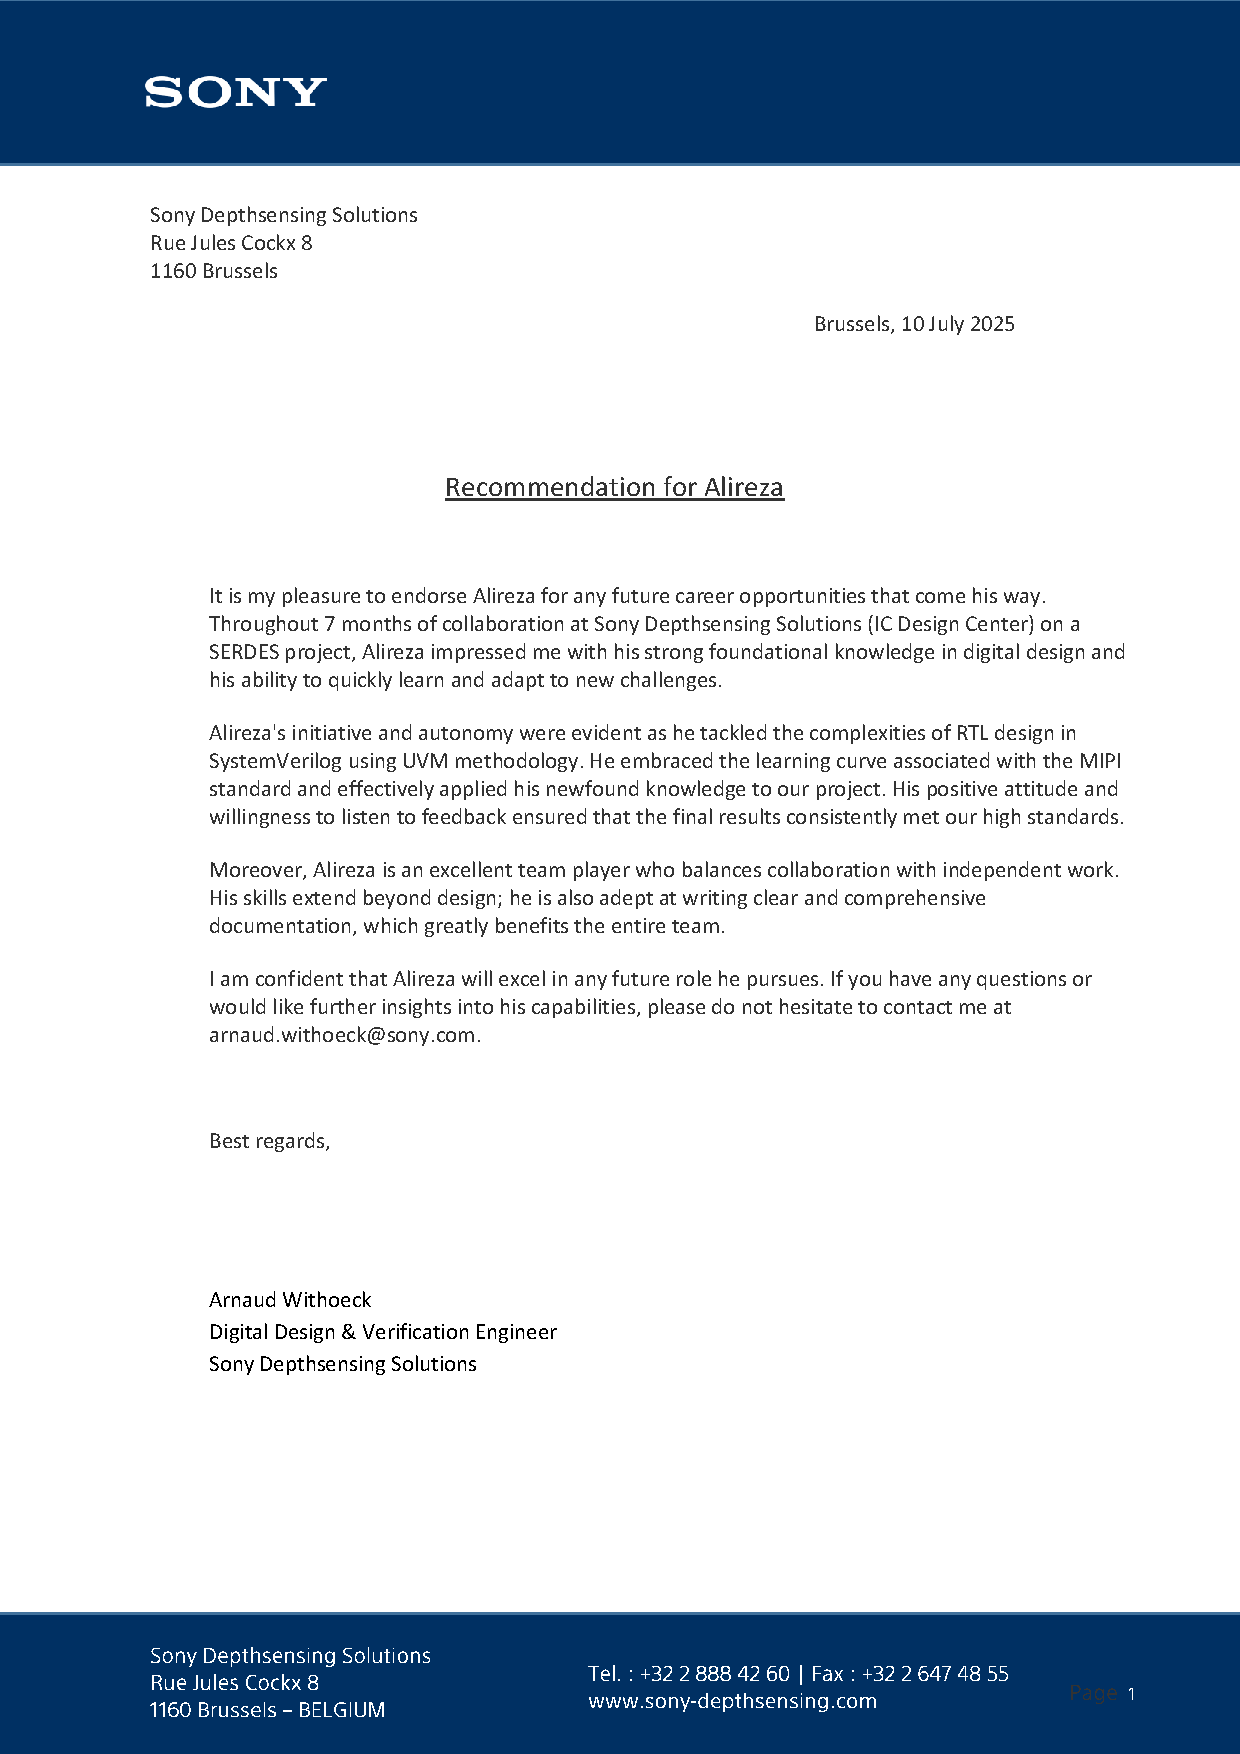
\includepdf[pages=-]{cv-sections/Sony.pdf}
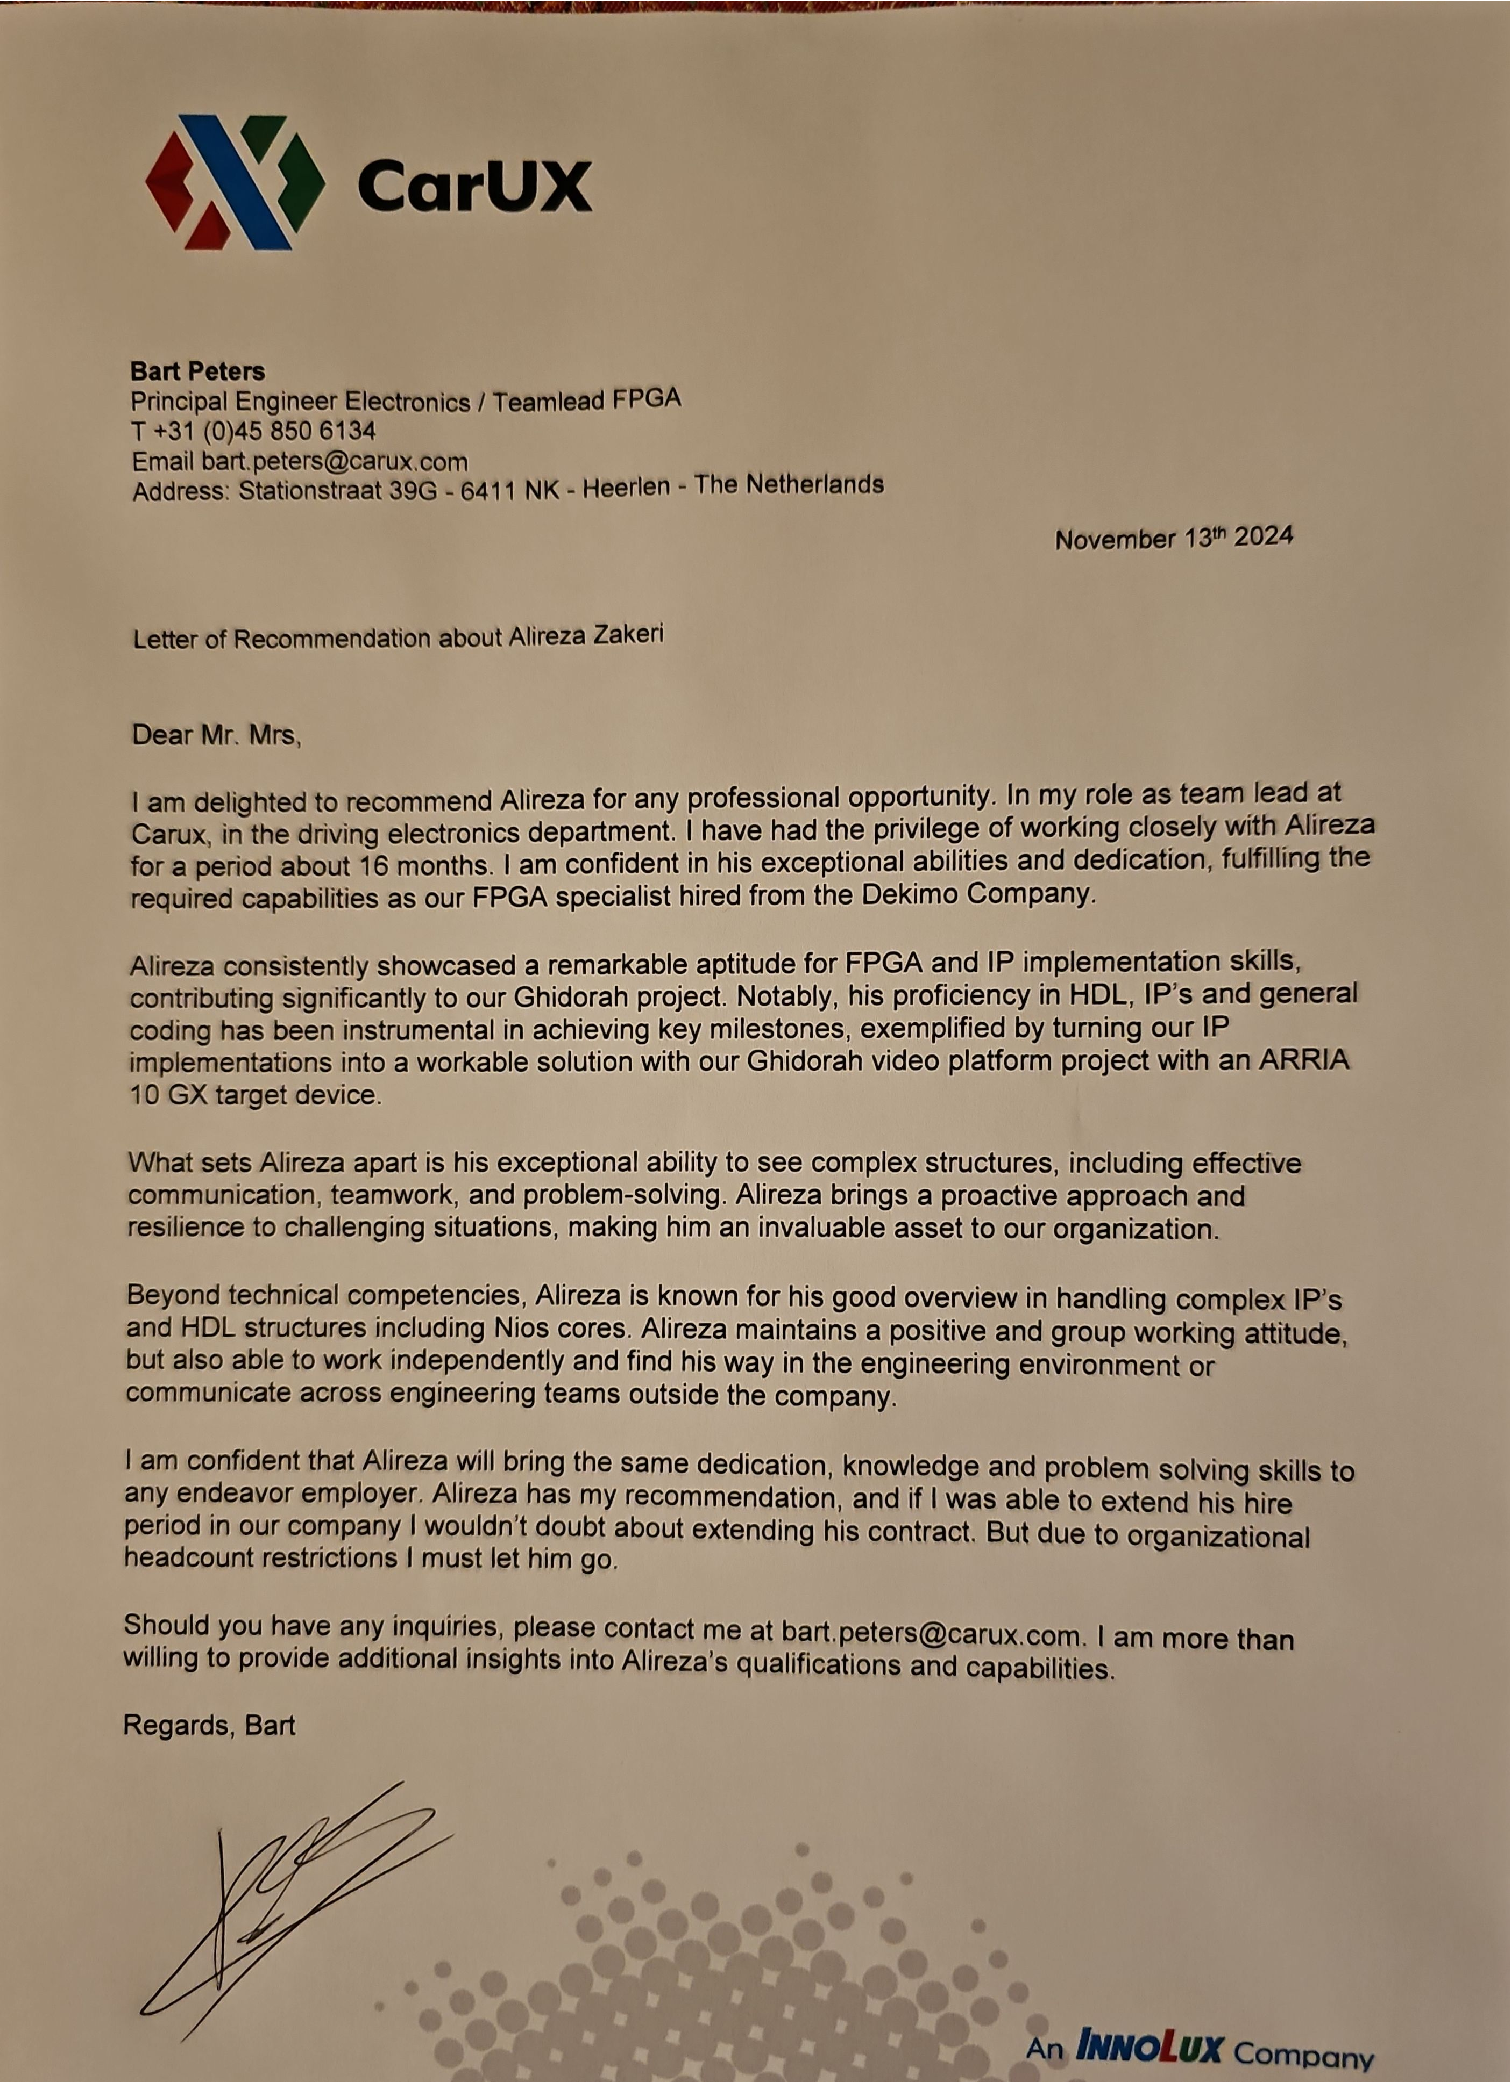
\includepdf[pages=-]{cv-sections/carux.pdf}

%%----------------------------------------------------------------------------------------
%	SECTION TITLE
%----------------------------------------------------------------------------------------

\cvsection{Extracurricular Activity}

%----------------------------------------------------------------------------------------
%	SECTION CONTENT
%----------------------------------------------------------------------------------------

\begin{cventries}

%------------------------------------------------

\cventry
{Core Member} % Affiliation/role
{B10S (B1t 0n the Security, Underground hacker team)} % Organization/group
{S.Korea} % Location
{Nov. 2011 - PRESENT} % Date(s)
{ % Description(s) of experience/contributions/knowledge
\begin{cvitems}
\item {Gained expertise in penetration testing areas, especially targeted on web application and software.}
\item {Participated on a lot of hacking competition and won a good award.}
\item {Held several hacking competitions non-profit, just for fun.}
\end{cvitems}
}

%------------------------------------------------

\cventry
{Member} % Affiliation/role
{WiseGuys (Hacking \& Security research group)} % Organization/group
{S.Korea} % Location
{Jun. 2012 - PRESENT} % Date(s)
{ % Description(s) of experience/contributions/knowledge
\begin{cvitems}
\item {Gained expertise in hardware hacking areas from penetration testing on several devices including wireless router, smartphone, CCTV and set-top box.}
\item {Trained wannabe hacker about hacking technique from basic to advanced and ethics for white hackers by hosting annual Hacking Camp.}
\end{cvitems}
}

%------------------------------------------------

\cventry
{Core Member \& President at 2013} % Affiliation/role
{PoApper (Developers' Network of POSTECH)} % Organization/group
{Pohang, S.Korea} % Location
{Jun. 2010 - PRESENT} % Date(s)
{ % Description(s) of experience/contributions/knowledge
\begin{cvitems}
\item {Reformed the society focusing on software engineering and building network on and off campus.}
\item {Proposed various marketing and network activities to raise awareness.}
\end{cvitems}
}

%------------------------------------------------

\cventry
{Member} % Affiliation/role
{PLUS (Laboratory for UNIX Security in POSTECH)} % Organization/group
{Pohang, S.Korea} % Location
{Sep. 2010 - Oct. 2011} % Date(s)
{ % Description(s) of experience/contributions/knowledge
\begin{cvitems}
\item {Gained expertise in hacking \& security areas, especially about internal of operating system based on UNIX and several exploit techniques.}
\item {Participated on several hacking competition and won a good award.}
\item {Conducted periodic security checks on overall IT system as a member of POSTECH CERT.}
\item {Conducted penetration testing commissioned by national agency and corporation.}
\end{cvitems}
}

%------------------------------------------------

\cventry
{Member} % Affiliation/role
{MSSA (Management Strategy Club of POSTECH)} % Organization/group
{Pohang, S.Korea} % Location
{Sep. 2013 - PRESENT} % Date(s)
{ % Description(s) of experience/contributions/knowledge
\begin{cvitems}
\item {Gained knowledge about several business field like Management, Strategy, Financial and marketing from group study.}
\item {Gained expertise in business strategy areas and inisght for various industry from weekly industry analysis session.}
\end{cvitems}
}

%------------------------------------------------

\end{cventries}
%%----------------------------------------------------------------------------------------
%	SECTION TITLE
%----------------------------------------------------------------------------------------

\cvsection{Honors \& Awards}

%----------------------------------------------------------------------------------------
%	INTERNATIONAL SUBSECTION
%----------------------------------------------------------------------------------------

\cvsubsection{International}

%------------------------------------------------

\begin{cvhonors}

%------------------------------------------------

\cvhonor
{Finalist} % Award
{DEFCON 22nd CTF Hacking Competition World Final} % Event
{Las Vegas, U.S.A} % Location
{2014} % Date(s)

%------------------------------------------------

\cvhonor
{Finalist} % Award
{DEFCON 21st CTF Hacking Competition World Final} % Event
{Las Vegas, U.S.A} % Location
{2013} % Date(s)

%------------------------------------------------

\cvhonor
{Finalist} % Award
{DEFCON 19th CTF Hacking Competition World Final} % Event
{Las Vegas, U.S.A} % Location
{2011} % Date(s)

%------------------------------------------------

\cvhonor
{6th Place} % Award
{SECUINSIDE Hacking Competition World Final} % Event
{Seoul, S.Korea} % Location
{2012} % Date(s)

%------------------------------------------------

\end{cvhonors}

%----------------------------------------------------------------------------------------
%	DOMESTIC SUBSECTION
%----------------------------------------------------------------------------------------

\cvsubsection{Domestic}

%------------------------------------------------

\begin{cvhonors}

%------------------------------------------------

\cvhonor
{3rd Place} % Award
{WITHCON Hacking Competition Final} % Event
{Seoul, S.Korea} % Location
{2015} % Date(s)

%------------------------------------------------

\cvhonor
{Silver Prize} % Award
{KISA HDCON Hacking Competition Final} % Event
{Seoul, S.Korea} % Location
{2013} % Date(s)

%------------------------------------------------

\cvhonor
{2nd Award} % Award
{HUST Hacking Festival} % Event
{S.Korea} % Location
{2013} % Date(s)

%------------------------------------------------

\cvhonor
{3rd Award} % Award
{HUST Hacking Festival} % Event
{S.Korea} % Location
{2010} % Date(s)


%------------------------------------------------

\cvhonor
{3rd Award} % Award
{Holyshield 3rd Hacking Festival} % Event
{S.Korea} % Location
{2012} % Date(s)

%------------------------------------------------

\cvhonor
{2nd Award} % Award
{Holyshield 3rd Hacking Festival} % Event
{S.Korea} % Location
{2011} % Date(s)

%------------------------------------------------

\cvhonor
{5th Place} % Award
{PADOCON Hacking Competition Final} % Event
{Seoul, S.Korea} % Location
{2011} % Date(s)

%------------------------------------------------

\end{cvhonors}
%%----------------------------------------------------------------------------------------
%	SECTION TITLE
%----------------------------------------------------------------------------------------

\cvsection{Presentation}

%----------------------------------------------------------------------------------------
%	SECTION CONTENT
%----------------------------------------------------------------------------------------

\begin{cventries}

%------------------------------------------------

\cventry
{Presenter for <DEFCON 20th : The way to go to Las Vegas>} % Role
{6th CodeEngn (Reverse Engineering Conference)} % Event
{Seoul, S.Korea} % Location
{Jul. 2012} % Date(s)
{ % Description(s)
\begin{cvitems}
\item {Introduced CTF (Capture the Flag) hacking competition and advanced techniques and strategy for CTF}
\end{cvitems}
}

%------------------------------------------------

\cventry
{Presenter for <Metasploit 101>} % Role
{6th Hacking Camp - S.Korea} % Event
{S.Korea} % Location
{Sep. 2012} % Date(s)
{ % Description(s)
\begin{cvitems}
\item {Introduced basic procedure for penetration testing and how to use Metasploit}
\end{cvitems}
}

%------------------------------------------------

\end{cventries}
%%----------------------------------------------------------------------------------------
%	SECTION TITLE
%----------------------------------------------------------------------------------------

\cvsection{Writing}

%----------------------------------------------------------------------------------------
%	SECTION CONTENT
%----------------------------------------------------------------------------------------

\begin{cventries}

%------------------------------------------------

\cventry
{Founder \& Writer} % Role
{A Guide for Developers in Start-up} % Title
{Facebook Page} % Location
{Jan. 2015 - PRESENT} % Date(s)
{ % Description(s)
\begin{cvitems}
\item {Drafted daily news for developers in Korea about IT technologies, issues about start-up.}
\end{cvitems}
}

%------------------------------------------------

\cventry
{Undergraduate Student Reporter} % Role
{AhnLab} % Title
{S.Korea} % Location
{Oct. 2012 - Jul. 2013} % Date(s)
{ % Description(s)
\begin{cvitems}
\item {Drafted reports about IT trends and Security issues on AhnLab Company magazine.}
\end{cvitems}
}

%------------------------------------------------

\end{cventries}
%%----------------------------------------------------------------------------------------
%	SECTION TITLE
%----------------------------------------------------------------------------------------

\cvsection{Program Committees}

%----------------------------------------------------------------------------------------
%	SECTION CONTENT
%----------------------------------------------------------------------------------------

\begin{cvhonors}

%------------------------------------------------

\cvhonor
{Organizer \& Co-director} % Position
{1st POSTECH Hackathon} % Committee
{S.Korea} % Location
{2013} % Date(s)
    
%------------------------------------------------

\cvhonor
{Staff} % Position
{7th Hacking Camp} % Committee
{S.Korea} % Location
{2012} % Date(s)

%------------------------------------------------

\cvhonor
{Problem Writer} % Position
{1st Hoseo University Teenager Hacking Competition} % Committee
{S.Korea} % Location
{2012} % Date(s)

%------------------------------------------------

\cvhonor
{Staff \& Problem Writer} % Position
{JFF(Just for Fun) Hacking Competition} % Committee
{S.Korea} % Location
{2012} % Date(s)

%------------------------------------------------

\end{cvhonors}

%----------------------------------------------------------------------------------------

\end{document}
